%
%~~
%~~  O Sistema Operacional KinOS
%~~
%

\chapter{O Sistema Operacional KinOS} \label{chap:sistema}
\index{sistema}

O principal objetivo do projeto � auxiliar o ensino de sistemas operacionais e da arquitetura ARM nas disciplinas de Sistemas Operacionais e Laborat�rio de Microprocessadores. Para tal, foi desenvolvido um \emph{microkernel}, apelidado de KinOS, cujas fun��es b�sicas s�o o chaveamento de \emph{threads} atrav�s de interrup��o de \emph{timer}, as chamadas de sistema, as rotinas de manipula��o de \emph{hardware}, fun��es de \emph{mutex} e um \emph{shell}.

% No codigo:
% Se todos os slots estiverem ocupados, ao se iniciar o 10o processo, o programa trava
% Fazer processos-exemplo
% -Exemplo de teste de seguran�a
% -Exemplo do mutex
% -Colocar teste onde fork retorna valores diferentes
% -Mostrar que depois de se criar dois processos; os dois estao com variaveis locais diferentes (duas threads rodando em cima de um mesmo aplicativo)

% Na monografia:
% Pr� t�rmino --------------------------
% Terminar:
% -Mutex
% -Inspira��o
% -Exemplos
% Colocar refer�ncias das apresenta��es
% Refazer numera��o do projeto

% P�s t�rmino --------------------------
% Colocar a referencia das se��es texto -> c�digo
% Emphasize essas variaveis: timer, microkernel, hardware, software, shell, assembly, threads, user, offset, link register, process counter, debug
% Revisar portugues no word
% Fazer revisao cruzada
% Ver se tem 'system call', 'processo' e 'mos'


% Delegar: 
% Colocar pesquisa inicial (ver tambem as referencias e documentos de acompanhamento iniciais)
% Kinoshita queria a parte da SWI bem documentada

\section{Organiza��o do c�digo}

A estrutura de arquivos do projeto pode ser vista na figura \ref{arquivos}. Pode-se dividi-lo em cinco partes: 

\begin{figure}[!ht]
\centering 
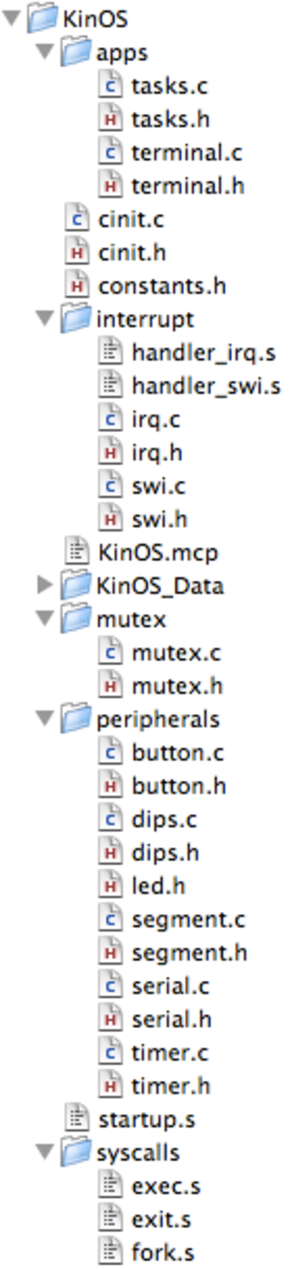
\includegraphics[width=4cm]{figuras/arquivos.pdf}
\caption{Estrutura de arquivos. \label{arquivos}}
\end{figure}

\begin{itemize}
\item{\textbf{Raiz} Arquivos de inicializa��o da placa}
\item{\textbf{Pasta ``apps''} Programas que ser�o executados pelo \emph{microkernel}}
\item{\textbf{Pasta ``interrupt''} Rotinas de tratamento de interrup��o}
\item{\textbf{Pasta ``peripherals''} Rotinas de manipula��o de \emph{hardware}}
\item{\textbf{Pasta ``syscalls''} Chamadas de sistema}
\item{\textbf{Pasta ``mutex''} Rotinas do \emph{mutex}}
\end{itemize}

A pasta KinOS\_Data n�o � considerada parte do projeto pois � utilizada pelo CodeWarrior para o armazenamento do c�digo compilado.

\subsection{Raiz}

Os arquivos encontrados na raiz do projeto s�o respons�veis pela inicializa��o da placa e pela declara��o de constantes globais.  O arquivo startup.s cont�m a chamada inicial do \emph{microkernel}, onde toda parte de inicializa��o em \emph{assembly} � feita. J� o arquivo cinit.c tamb�m cont�m a parte de inicializa��o, por�m, o c�digo est� escrito em C. Finalmente, o arquivo constants.h � respons�vel por armazenar as constantes que s�o utilizadas em todo o projeto.

\subsection{Pasta ``apps''}

No arquivo tasks.c, v�rias fun��es s�o declaradas, onde cada declara��o � considerada uma \emph{thread} pelo \emph{microkernel}. Mais � frente, na se��o \ref{cap:processos}, os programas exemplo ser�o descritos com mais detalhe. J� no arquivo terminal.c, h� o \emph{shell} do sistema.

\subsection{Pasta ``interrupt''}

Todas as rotinas que tratam e instalam interrup��es -- tanto de \emph{hardware} quanto de \emph{software} -- est�o localizadas nesta pasta. O arquivo handler\_irq.s cont�m a rotina em \emph{assembly} que trata das interrup��es de \emph{hardware}, as encaminha para a rotina espec�fica de acordo com a sua fonte e faz o chaveamento de \emph{threads}. O arquivo irq.c cont�m uma �nica rotina, que realiza a instala��o da rotina de tratamento de interrup��o tanto de \emph{hardware} quanto de \emph{software}. A rotina de tratamento de interrup��o de \emph{software} � feita no arquivo handler\_swi.s, que identifica o tipo de interrup��o e encaminha para alguma das chamadas de sistema, encontradas em swi.c.

\subsection{Pasta ``peripherals''}

As rotinas de inicializa��o e controle dos perif�ricos se encontram todas nesta pasta. As do bot�o est�o no arquivo button, da chave DIP no arquivo dips, do display de sete segmentos em segment, dos LEDs em led e do \emph{timer} em timer.

\subsection{Pasta ``syscalls''}

As chamadas de sistema est�o escritas em \emph{assembly} e se encontram em tr�s arquivos, uma para cada chamada. S�o elas as chamadas fork, exec e exit.

\subsection{Pasta ``mutex''}

No arquivo mutex h� apenas as fun��es que permitem a exclus�o m�tua de c�digo por espera ativa, feita atrav�s de um \emph{mutex}.

\section{Estruturas de dados}

A fim de se facilitar a programa��o e o entendimento do projeto, foram criadas duas estruturas de dados que s�o acessadas em \emph{assembly}. A primeira, o \emph{Process Control Block} � respons�vel pelo armazenamento do estado de uma \emph{thread}. J� o "vetor de \emph{threads}" realiza o controle de quais \emph{threads} est�o ativas.

\subsection{Process Control Block} \label{sub:PCB}

O \emph{Process Control Block} (ou simplesmente PCB) � um estrutura de dados que guarda todas as informa��es de uma \emph{thread} que aguarda para ser executada enquanto outras est�o ativas. H� um PCB para cada uma das nove \emph{threads} e cada um ocupa 68 bytes. Ou seja, o espa�o total ocupado pelos PCBs � de 9 $\cdot$ 68 = 612 bytes. Estes 68 bytes est�o estruturados como explicitado na figura \ref{pcb}. Cada posi��o da tabela ocupa uma palavra (4 bytes). A primeira posi��o � em (base do PCB - 4), a segunda em (base do PCB - 8) e assim por diante. Como pode-se observar pela figura, as posi��es 1 a 15 ((base do PCB - 4) a (base do PCB - 60)) armazenam o conte�do dos registradores r0 a r14 do modo \emph{user} em ordem inversa. A posi��o 16 (base do PCB - 64) armazena o \emph{link register} do modo IRQ, ou seja, o endere�o de retorno da interrup��o. Finalmente, a posi��o 17 armazena o registrador de estado do modo \emph{user}. Estes registradores armazenados permitem estabelecer um retrato preciso do estado da \emph{thread} quando houve o chaveamento e permite tamb�m que este estado seja restabelecido quando for o turno desta \emph{thread} voltar a ser executada. A estrutura tem seu espa�o reservado no arquivo handler\_irq.s, e � nomeado com a vari�vel process\_control\_block, que indica a base da estrutura. Cada um dos PCBs est� logo a seguir do anterior. Por exemplo, a base do primeiro PCB est� em (process\_control\_block - 68), do segundo em (process\_control\_block - 2 $\cdot$ 68) e assim por diante.

\begin{figure}[!ht]
\centering 
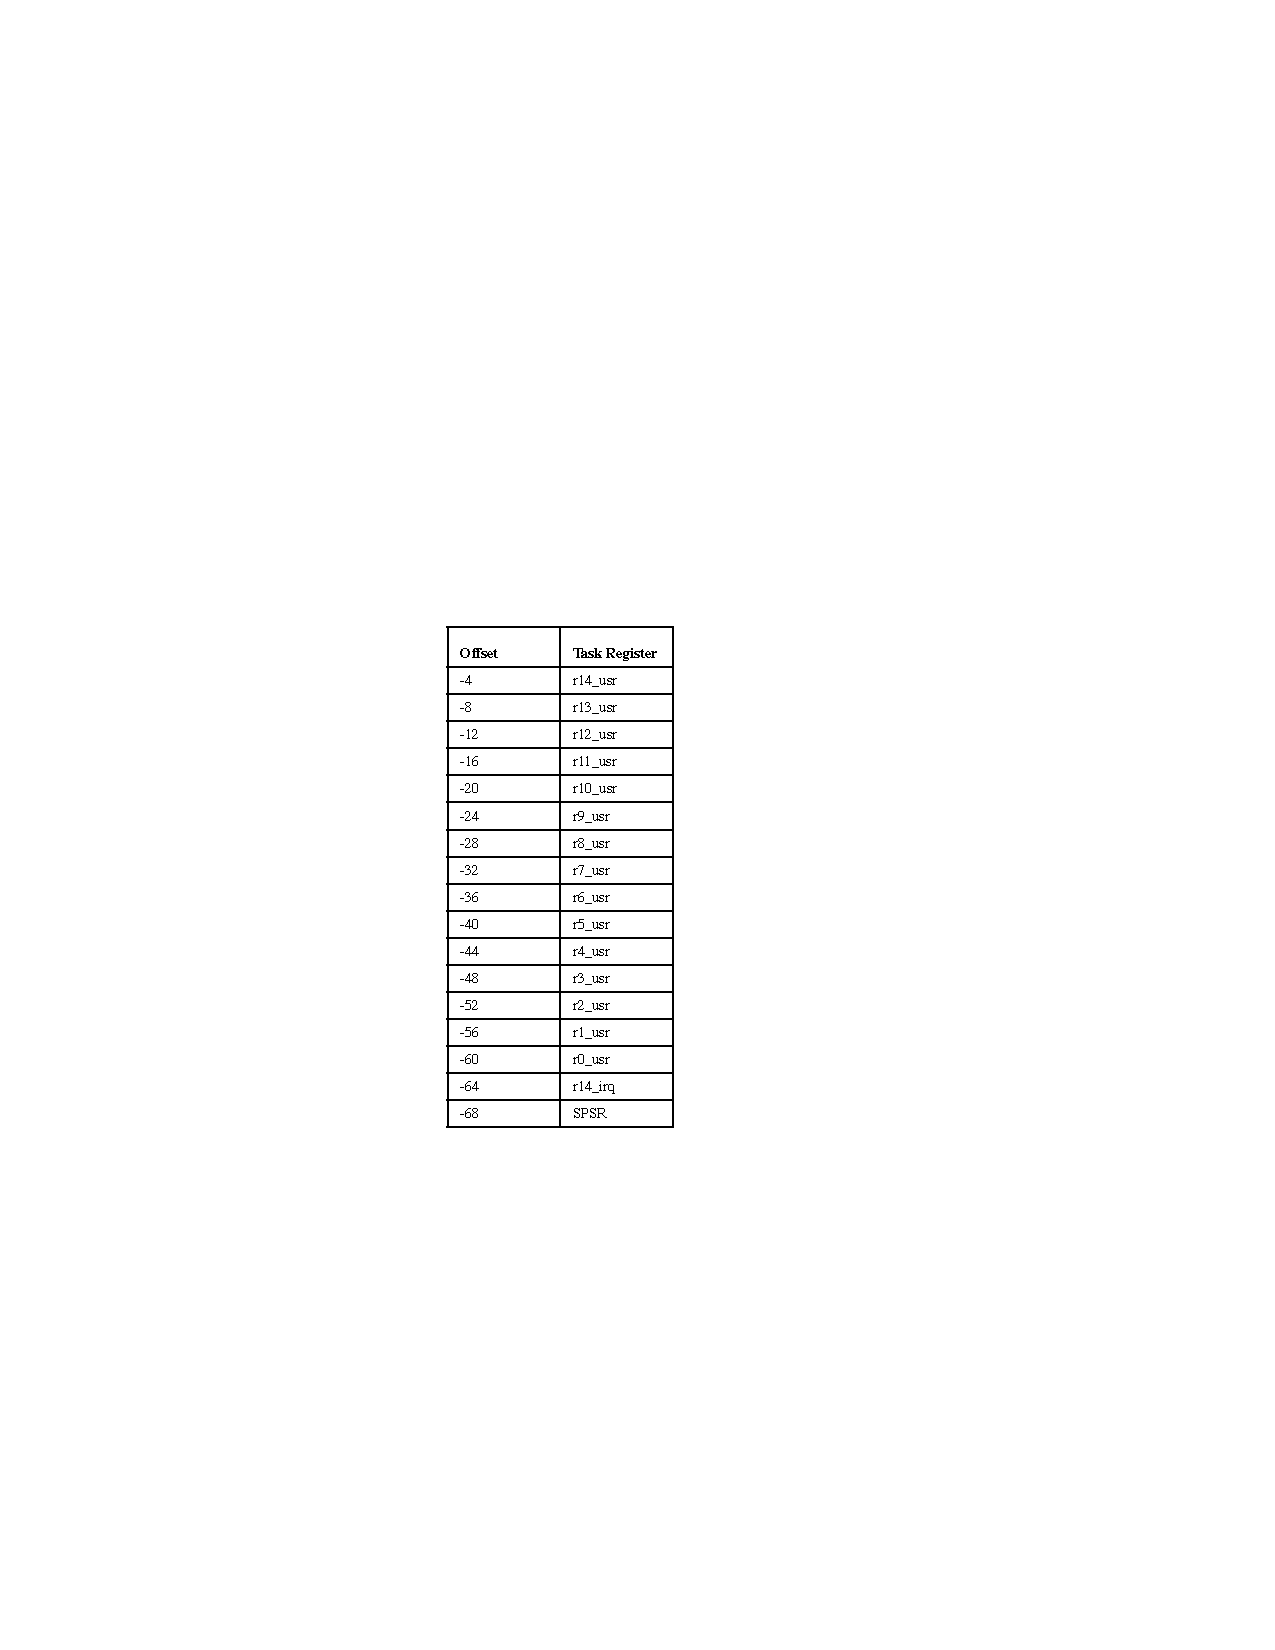
\includegraphics[height=10cm]{figuras/pcb.pdf}
\caption{Estrutura de dados do PCB. Fonte: \cite{Sloss2001} \label{pcb}}
\end{figure}

\subsection{Vetor de \emph{threads}}

O vetor de \emph{threads} � uma lista que armazena quais das \emph{threads} est�o ativas e quais n�o est�o, a fim de se identificar quais devem ser colocadas em execu��o. Cada identificador ocupa 4 bytes, e pode ter os valores 0 (inativo) ou 1 (ativo). Como h� 9 \emph{threads}, o tamanho deste vetor � de 4 $\cdot$ 9 = 36 bytes. Seu espa�o � reservado no arquivo handler\_irq.s, com o nome de thread\_array. No exemplo na figura \ref{vetor} pode-se ver que as \emph{threads} 1, 2 e 4 est�o ativas, enquanto que as outras n�o est�o.\\

\begin{figure}[!ht]
\centering 
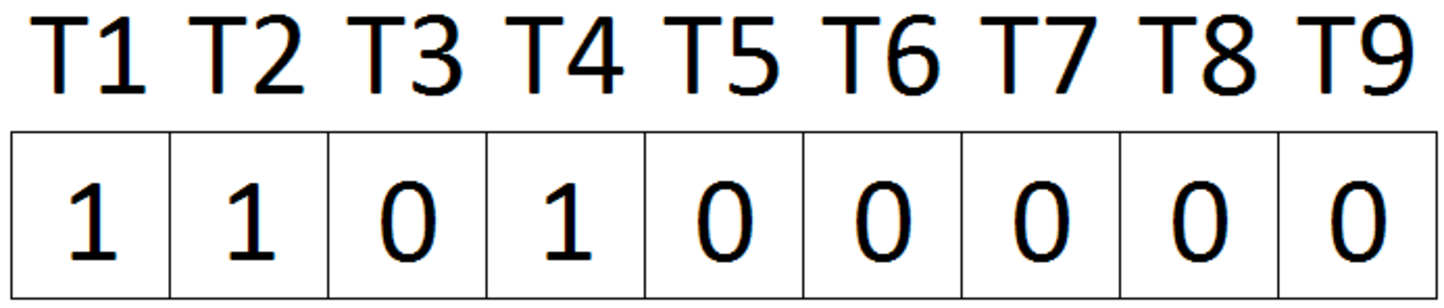
\includegraphics[width=7.5cm]{figuras/vetorThreads.pdf}
\caption{Vetor de \emph{threads}. \label{vetor}}
\end{figure}

\section{Configura��o de \emph{hardware} e \emph{software}}

Nesta se��o s�o apresentados os modos como o \emph{hardware} e o \emph{software} descritos anteriormente s�o utilizados. Ser� indicado como foi feito o particionamento da mem�ria, a utiliza��o dos modos do processador e os modos de teste do c�digo. 

\subsection{Mem�ria}

A mem�ria vol�til da placa foi estruturada como indicado na figura \ref{memoria}. Para todo espa�o das pilhas, programas, c�digo, vetor de interrup��es e �rea de dados, o espa�o dispon�vel � de 128KB (de 0x0 a 0x20000). Como p�de ser visto na se��o \ref{sub:interrupcoes}, a mem�ria entre 0x0 e 0x20 cont�m o vetor de interrup��es e deve ser reservado. A pilha do modo SVC come�a no endere�o 0x7F80, cresce para baixo e n�o deve invadir a �rea reservada para o vetor de interrup��o. J� a pilha do modo IRQ, come�a no endere�o 0x8000, tamb�m cresce para baixo e n�o deve invadir o espa�o reservado para a pilha do modo SVC. O c�digo do \emph{kernel} e dos programas come�a no endere�o 0x8000, mas ao contr�rio da pilha do modo SVC, cresce para cima. Logo ap�s o c�digo, temos uma �rea reservada para os dados globais. Finalmente, as pilhas do modo \emph{user} come�am no endere�o 0x20000 e crescem para baixo. Cada uma tem um offset relativo � anterior de 4048 bytes.

\begin{figure}[!ht]
\centering 
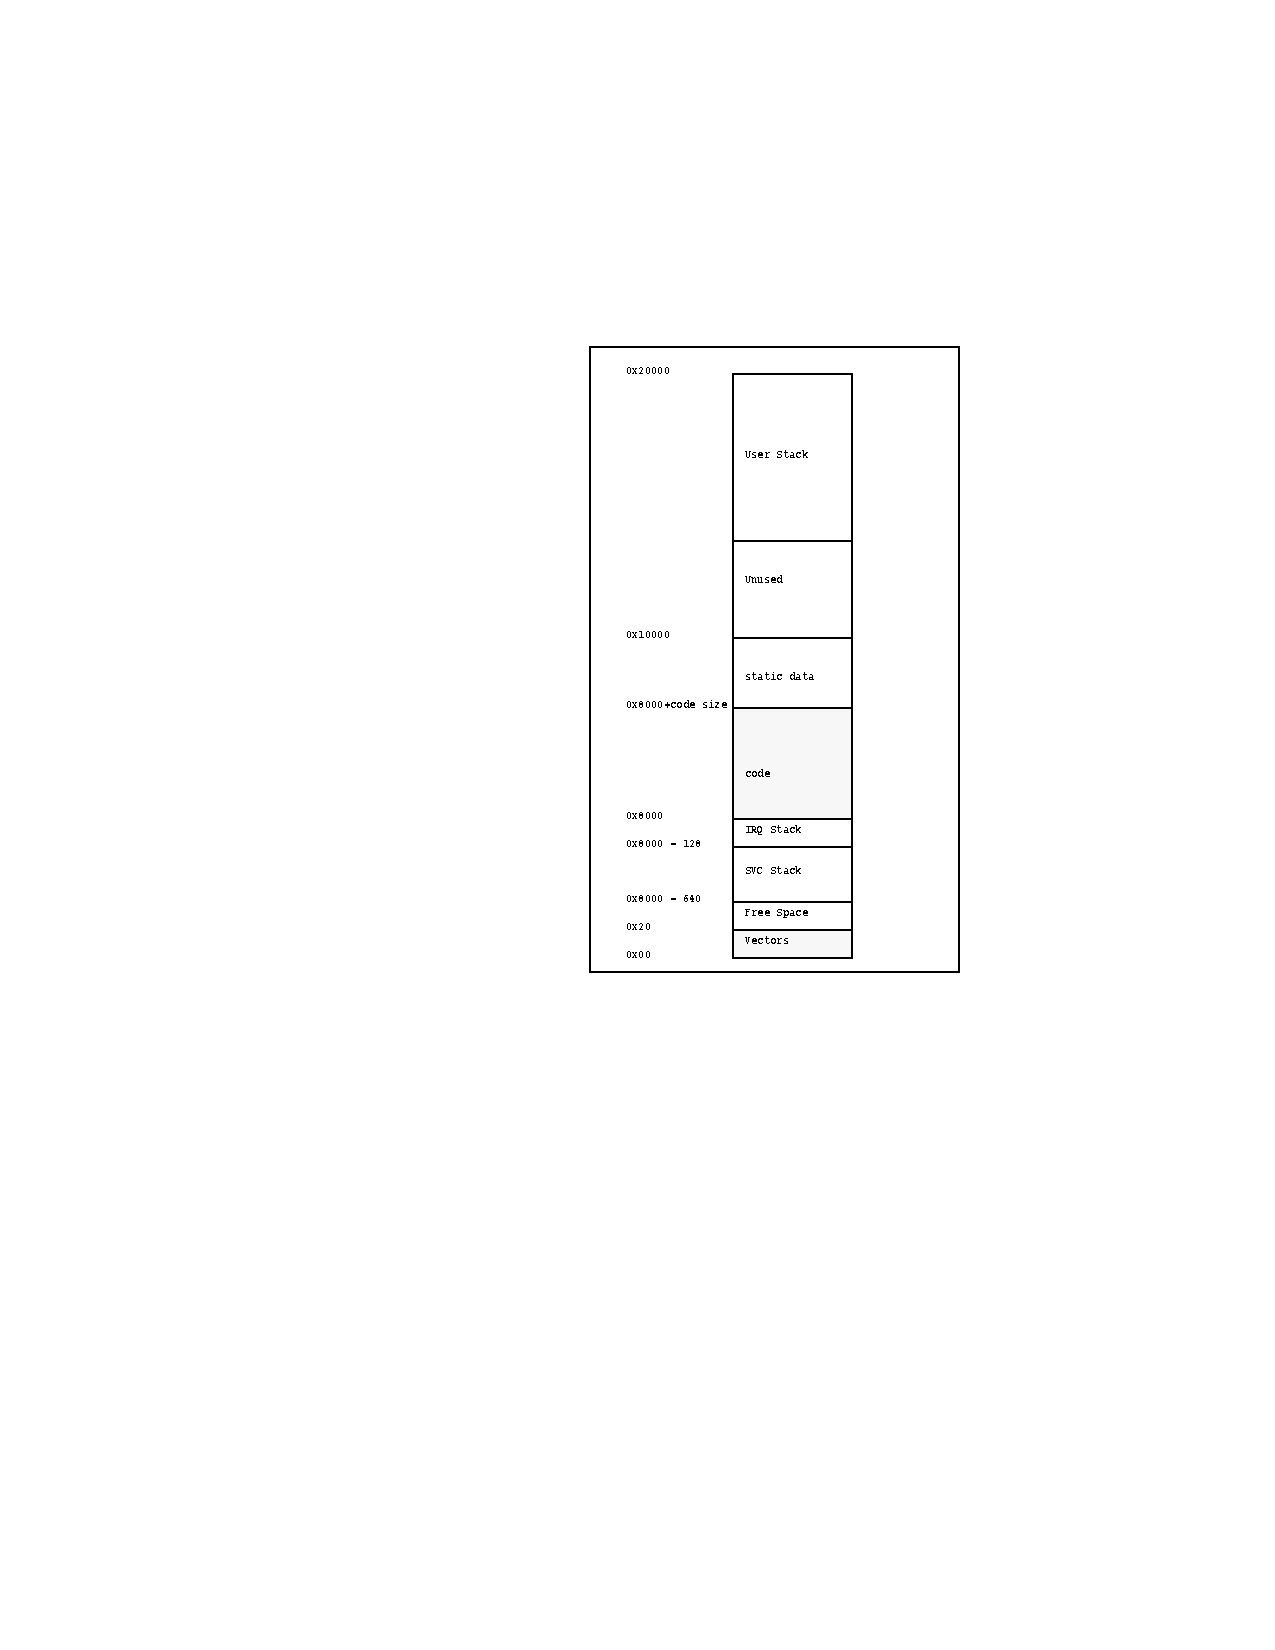
\includegraphics[height=13cm]{figuras/memoria.pdf}
\caption{Estrutura da mem�ria. Fonte: \cite{Sloss2001} \label{memoria}}
\end{figure}

\subsection{Modos do processador}

Dentre os sete modos do processador, apenas quatro deles s�o utilizados: o modo de usu�rio (\emph{user}), o modo de servi�o (SVC), o modo de sistema (SYS) e o modo de interrup��o (IRQ). O primeiro � o modo n�o privilegiado no qual as \emph{threads} s�o executadas. O segundo, � o modo de inicializa��o do \emph{kernel} e de execu��o das chamadas de sistema, que � privilegiado. J� o terceiro, � id�ntico ao modo de usu�rio, mas com privil�gios. Ele � utilizado na inicializa��o do sistema para definir a pilha do modo de usu�rio. Finalmente, o quarto � um modo que tamb�m � privilegiado, mas que � usado quando h� interrup��es de \emph{hardware} e portanto, � usado quando h� o chaveamento de \emph{threads} (interrup��o de \emph{timer}) ou qualquer outra interrup��o que n�o a de \emph{software}. � importante ressaltar que os modos privilegiados quando chamados por interrup��o desabilitam outras interrup��es. Isso bloqueia interrup��es aninhadas, essencial para o funcionamento do c�digo.

\subsection{Modos de teste}

Depurar o c�digo com a placa n�o � poss�vel em todas as situa��es. Quando o c�digo que est� sendo executado est� dentro de uma regi�o onde as interrup��es est�o desabilitadas, como no c�digo de tratamento de interrup��o, n�o se pode faz�-lo. Para contornar tal problema, foi utilizado o emulador dispon�vel na IDE CodeWarrior, o ARMulator. Como ele foi desenvolvido para v�rios modelos de placa, utiliza endere�os de perif�ricos diferentes da placa Evaluator 7-T e n�o t�m o m�dulo Angel de \emph{debug}. Para manter a compatibilidade entre o emulador e a placa nas partes onde o c�digo se diferencia, como na inicializa��o do \emph{timer}, foram colocados ambos c�digos. A sele��o de qual dos dois ser� executado depende de uma vari�vel global emulator, que � declarada no arquivo constants.h. Caso seja 1, o c�digo executado � o do emulador, caso seja 0, o c�digo da placa com Angel e caso seja 2, o c�digo para a placa sem o Angel. Uma outra vantagem do c�digo no emulador � que ele permite com que ele possa ser testado sem a presen�a da placa.

\subsection{Angel}
\label{config:angel}
O Angel � um programa contido na ROM da placa que realiza a comunica��o entre a mesma e o computador que efetuou o upload do c�digo. Al�m de permitir com que o c�digo seja carregado na placa, o Angel realiza o processo de \emph{debug} do c�digo durante a execu��o. Para isso, deve haver uma comunica��o constante entre a placa e o computador, que � feita atrav�s de interrup��es. Uma vez que a placa � iniciada, o endere�o do vetor de interrup��es respons�vel pelas interrup��es de \emph{hardware} e se \emph{software} apontam para um endere�o pr�-estabelecido do Angel. 

Caso se queira adicionar alguma outra rotina de tratamento de interrup��es, como � o caso deste projeto, deve-se encadear o Angel (como ser� descrito na se��o \ref{init:install}) quando a rotina instalada n�o consegue tratar a interrup��o. Isto � necess�rio para que a comunica��o com a placa n�o seja perdida.

\section{Inicializa��o}

O in�cio do programa se d� no arquivo assembly statup.s. Nele, s�o feitas todas as opera��es que n�o podem ser feitas no c�digo em C, como a inicializa��o das pilhas ou a cria��o da tabela de threads. Ap�s esta etapa, h� a inicializa��o em C, feita no arquivo cinit.c, que inicializa perif�ricos, instala rotinas de tratamento e inicia a primeira thread em modo usu�rio. A rotina completa de inicializa��o pode ser vista no esquema da figura \ref{inicializacao}.

\begin{figure}[!ht]
\centering 
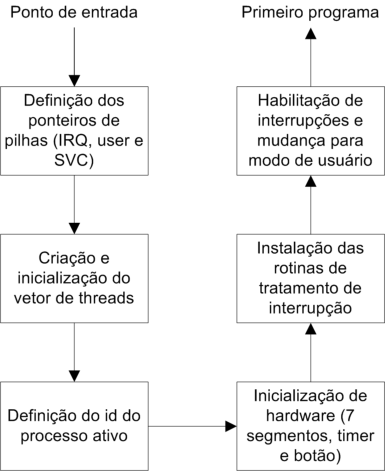
\includegraphics[height=10cm]{figuras/inicializacao.pdf}
\caption{Fluxograma de inicializa��o. \label{inicializacao}}
\end{figure}

\subsection{Ponto de entrada e tipo de c�digo}

O ponto de entrada do c�digo � indicado pela instru��o \verb|ENTRY|. Por padr�o, o compilador assume que o c�digo de entrada � ARM. Como descrito anteriormente, h� dois tipos de assembly, o ARM e o THUMB. No microkernel, � utilizado apenas c�digo ARM, j� que ele fornece mais instru��es e favorece a legibilidade. Um ponto negativo deste tipo de c�digo � seu maior espa�o ocupado na mem�ria, mas isso n�o vem a ser um grande problema, pois temos espa�o suficiente.

\subsection{Pilhas}

Antes de poder utilizar as pilhas � preciso que elas sejam inicializadas em cada um dos modos que vir�o a ser utilizados. Neste microkernel, s�o utilizados os modos de servi�o, usu�rio/sistema e de interrup��o. O modo como isto � feito � descrito abaixo:

\begin{lstlisting}
	MOV		r0,	#0xC0|0x12		; r0 = 0xC0 or 0x12 (0xC0 = IRQ disabled, 0x12 = IRQ mode)
	MSR		CPSR_c, r0			; status_register = r0
	MOV		sp, #0x8000			; stack pointer = 0x8000
\end{lstlisting}

A primeira instru��o copia para r0 o que ser� substitu�do no registrador de estado. Neste exemplo, est� se desabilitando as interrup��es e mudando o modo do processador para o modo de interrup��o. Em seguida, os dados do registrador r0 s�o colocados no registrador de estado. Uma vez que o estado foi alterado, pode-se mudar o ponteiro de pilha, que neste caso aponta para o endere�o 0x8000. Uma opera��o semelhante pode ser feita tanto no modo de servi�o quanto no modo de usu�rio, usando os endere�os de pilha indicados anteriormente. Por�m, se o estado for alterado para o modo de usu�rio fica imposs�vel de se alterar o estado novamente. Para se resolver este problema, ao inv�s de se mudar para o estado de usu�rio, muda-se para o estado de sistema. Este � o mesmo modo que o de usu�rio (usa a mesma pilha e registradores), mas permite que o modo seja alterado novamente.

\subsection{Vetor de threads e n�mero da thread}

O outro ponto importante da inicializa��o do c�digo em assembly � a cria��o do vetor de threads. Para tal, temos de definir que todos os processos exceto o primeiro s�o inicializados desabilitados. Isto � feito com o c�digo apresentado a seguir:

\begin{lstlisting}
	; Initializes the thread array with zeros (0 = thread disabled,
	; 1 = thread enabled)
	LDR		r0, =thread_array		; r0 = thread_array start address
	MOV		r1, #1					; r1 = 1
	STR		r1, [r0]				; address(r0) = r1
	MOV		r1, #0					; r1 = 0 (disabled)
	MOV		r2, #0					; r2 = 0
init_thread_array_loop
	ADD		r2, r2, #4				; r2 = r2 + 4
	CMP		r2, #36					; r2 = 36?
	BEQ		set_active_thread		; if yes, go to set_active_thread
	ADD		r3, r0, r2				; r3 = r0 + r2
	STR		r1, [r3]				; address(r3) = r1
	B		init_thread_array_loop	; return to init_thread_array_2
\end{lstlisting}

Nele, r0 armazena a base do vetor, que coincide com o espa�o relativo � primeira thread. r1 cont�m o dado que ser� colocado na posi��o de mem�ria. Na posi��o este valor � 1, e nos demais 0. r2 cont�m o offset que ser� somado � base para o c�lculo do endere�o absoluto, armazenado em r3. O algoritmo funciona inicialmente colocando 1 na base. Ap�s isso, entra em um loop que aumenta o offset de 4 em 4 e coloca 0 em todos os outros espa�os.

Ainda na inicializa��o em assembly, deve-se definir o n�mero da thread que est� sendo executada. Este dado � armazenado na vari�vel current\_thread\_id. Pode-se ver abaixo como � definido o id do primeiro processo para 1:

\begin{lstlisting}
LDR		r0, =current_thread_id	; r0 = current thread id address
MOV		r1, #1					; r1 = 1
STR		r1, [r0]				; current thread id = 1
\end{lstlisting}

Finalmente, a inicializa��o em C pode ser iniciada. A chamada � feita definindo como endere�o de retorno a fun��o C\_entry e colocando este mesmo endere�o no process counter.

\begin{lstlisting}
LDR 	lr, =C_Entry			; link register = C entry
MOV 	pc, lr					; process counter = C entry
\end{lstlisting}

\subsection{Perif�ricos}

Para alguns perif�rico da placa, como o display de sete segmentos, o timer e os bot�es, h� uma rotina de inicializa��o que os habilita e define suas configura��es. Suas chamadas s�o \verb|segment_init()|, \verb|timer_init()| e \verb|button_init()| respectivamente. Estas fun��es se encontram nos arquivos de cada um dos perif�ricos e s�o executadas logo no in�cio da etapa C do processo de inicializa��o da placa.

\subsection{Instala��o do tratamento de interrup��o}
\label{init:install}
Como descrito anteriormente, caso uma interrup��o de hardware ocorra, a instru��o no endere�o 0x18 � executada e caso seja uma interrup��o de software, a instru��o no endere�o 0x08. Toda vez que se reinicia a placa, s�o colocados nestes endere�os uma instru��o que realiza um desvio para a rotina Angel, descrita anteriormente. 

Por�m, se algum dos perif�ricos vai ser utilizado, a interrup��o gerada por esse perif�rico n�o deve desviada para o Angel, e sim para uma rotina adequada. Para poder identificar qual a origem da interrup��o e desviar para a rotina correta, devemos instalar uma nova rotina no vetor de interrup��es, substituindo o desvio para o Angel. A instala��o da rotina se d� atrav�s do desvio para a tal rotina. Todavia, n�o se pode apenas descartar o endere�o do Angel, j� que caso n�o se identifique a origem da interrup��o, ainda deve-se desviar para ele. Este processo pode ser observado na figura \ref{chain}. Nele, \emph{Handler2} � a rotina de tratamento de interrup��es, e \emph{Handler1} � o Angel.

A instala��o da rotina de tratamento de interrup��o � a mesma para interrup��es de hardware e de software se d� abaixo:

\begin{lstlisting}
/* Angel branch instruction */
unsigned Angel_branch_instruction;
/* Angel instruction */
unsigned *Angel_address;
/* Getting Angel branch instruction */		
Angel_branch_instruction  = *vector_address;
/* Separate the instruction from the address */
Angel_branch_instruction ^= 0xe59ff000;
/* Calculating absolute address */
Angel_address = (unsigned *) ((unsigned)vector_address + Angel_branch_instruction + 0x8);
/* Store address in the propoer position */
if ((unsigned)vector_address == 0x18) {
	Angel_IRQ_Address = *Angel_address;
}
else {
	Angel_SWI_Address = *Angel_address;
}
/* Inserting handler instruction in the vector table */
*Angel_address = handler_routine_address;
\end{lstlisting}

Os par�metros de entrada desta fun��o s�o \verb|handler_routine_address|, o endere�o da rotina de tratamento de interrup��o e \verb|vector_address|, um ponteiro para a posi��o no vetor de interrup��es onde ser� instalada a rotina. Sucintamente, o que esta rotina realiza � obter a instru��o que est� em \verb|vector_address|, aplica uma m�scara � rotina para obter apenas o endere�o e o salva em uma das vari�veis: \verb|Angel_IRQ_Address| caso se esteja instalando a rotina de interrup��o de hardware ou \verb|Angel_SWI_Address| caso seja a de software, al�m de colocar a nova instru��o no vetor de interrup��es. 

Um fator importante que deve ser ressaltado a import�ncia do Angel quando se est� usando a placa. Como j� descrito anteriormente, o Angel se utiliza das interrup��es de hardware e software para se comunicar com a placa. Portanto, se apenas modificarmos o c�digo e substituirmos a instru��o que est� contida no vetor de interrup��o, essa comunica��o n�o se realiza e tanto a placa quanto o programa de debugger travam. Para solucionarmos este problema, devemos passar para a rotina de tratamento de interrup��o os endere�os que estavam anteriormente no vetor de interrup��o, para o caso da interrup��o ser do Angel, a rotina correta ser executada. J� no caso em que o c�digo � apenas simulado no emulador, n�o � preciso armazenar o endere�o do Angel.

\begin{figure}[!ht]
\centering 
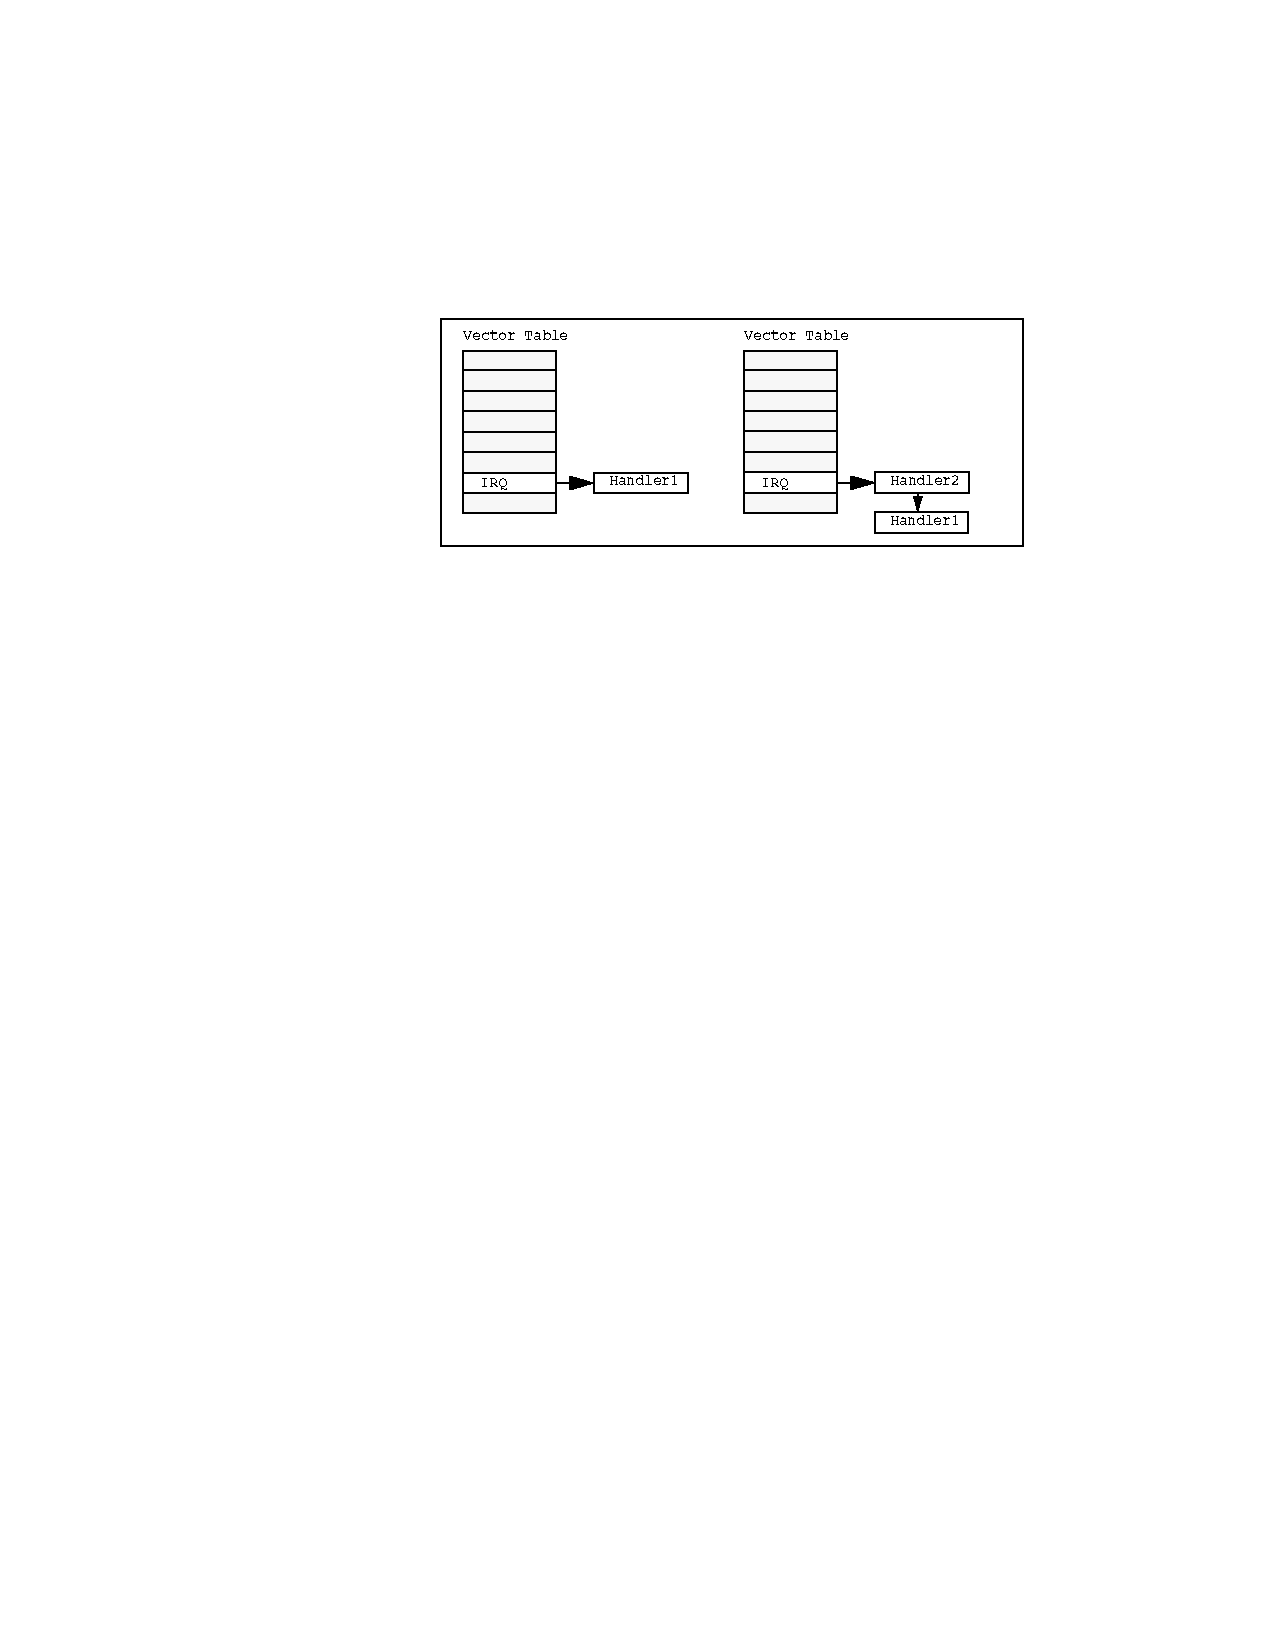
\includegraphics[width=13cm]{figuras/chain.pdf}
\caption{Encadeamento de interrup��es. Fonte: \cite{Sloss2001} \label{chain}}
\end{figure}

\subsection{Interrup��o de timer}

A interrup��o de timer � utilizada neste projeto para realizar o chaveamento entre as threads. Uma vez que haja a interrup��o, o estado da thread atual � salva e a pr�xima thread � colocada em processamento. Para utiliz�-la, devemos tanto habilitar quanto iniciar o timer. Essas tarefas s�o executadas com duas rotinas, sendo que a primeira j� foi descrita anteriormente. J� o in�cio do timer � dado pela fun��o \verb|timer_start()|.

\subsection{Habilitando interrup��es}

O �ltimo passo antes de se come�ar a executar o c�digo do primeiro programa � habilitar simultaneamente o modo de usu�rio e as interrup��es. Como isso s� pode ser feito por c�digo assembly, temos de usar a instru��o especial de C \_\_asm, conforme o exemplo abaixo

\begin{lstlisting}
__asm {
	MOV		r1,	#0x40|0x10
	MSR 	CPSR_c, r1
}
\end{lstlisting}

O registrador r1 recebe 0x40, que indica a habilita��o das interrup��es e 0x10 que altera para o modo de usu�rio. Logo em seguida, o conte�do deste registrador � passado para o registrador de estado. Finalmente, o primeiro programa � chamado com a fun��o \verb\shell()\.


\section{Chaveamento de processos}

O chaveamento de processos � realizado inteiramente com o assembly escrito no arquivo handler\_irq.s. Ele consiste em sete passos, indicados na figura \ref{chaveamento}.

\begin{figure}[!ht]
\centering 
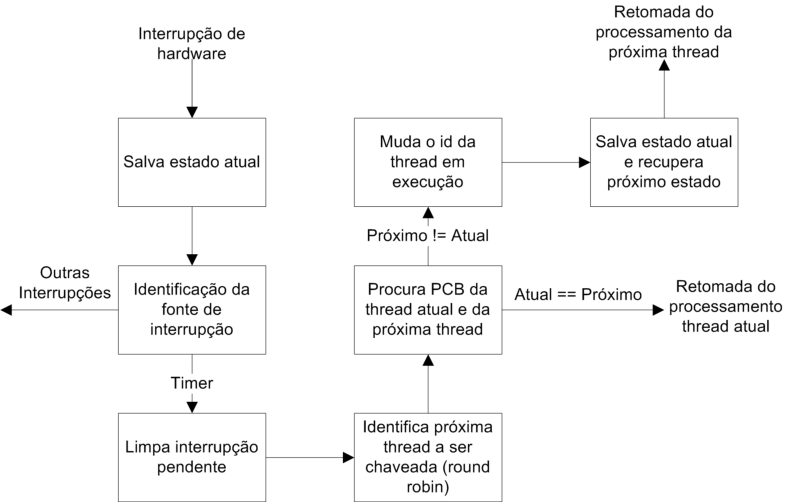
\includegraphics[width=15.5cm]{figuras/chaveamento.pdf}
\caption{Chaveamento de processos. \label{chaveamento}}
\end{figure}

\subsection{Identifica��o da interrup��o}

\begin{lstlisting}
STMFD	sp!, {r0 - r3, lr}		; Stacking r0 to r3 and the link register
LDR 	r0, IRQStatus	 		; r0 = irq type address
LDR 	r0, [r0]				; r0 = irq type
TST 	r0, #0x0400				; irq type == 0x0400?
BNE		handler_timer 			; If yes, go to handler_timer
TST		r0, #0x0001				; irq type = 0x0001?
BNE		handler_button			; If yes, go to handler_button
LDMFD	sp!, {r0 - r3, lr}		; If it is not any of them, restore r0-r3 and lr
LDR 	pc, Angel_IRQ_Address	; and branch to the Angel routine
\end{lstlisting}

Uma vez que h� a interrup��o de timer, a chamada de interrup��o de hardware que se encontra no vetor de interrup��o � executada. Durante a instala��o da rotina de tratamento de interrup��o de hardware, colocou-se nesta posi��o a rotina handler\_board\_angel caso se estivesse usando a placa com o Angel, a rotina handler\_board\_no\_angel caso se estivesse usando a placa sem o Angel ou a rotina handler\_emulator caso estivesse usando o emulador. A direren�a � que enquanto a primeira e a segunda tentam identificar qual a fonte de interrup��o, a terceira j� assume que a fonte � o timer, j� que n�o h� outros perif�ricos no emulador. Deve-se armazenar toda informa��o contida nos registradores que sao alterados durante o processo de tratamento de interrup��o. Para tal, empilhamos os valores dos registradores r0 a r3, usados durante a rotina de chaveamento, a fim de que nenhum dado se perca durante o processo.

No caso do uso da placa, a fonte da interrup��o se encontra no endere�o 0x03ff4004, identificado com a vari�vel \verb|INTPND|. Se o valor contido neste endere�o � 0x0400, a fonte foi uma interrup��o de timer, caso seja 0x0001, a fonte foi o bot�o da placa e caso contr�rio, a fonte foi o Angel. No primeiro caso, h� um desvio para a rotina \verb|handler_timer|, no segundo para a rotina \verb|handler_button| e na terceira, para o endere�o salvo durante a instala��o de rotina de tratamento.

\subsection{Limpeza da interrup��o de timer}

Quando � identificada a interrup��o de timer, deve-se limpar a interrup��o de timer, a fim de que ele possa interromper novamente no futuro. Para tal, executa-se a rotina timer\_irq, encontrada no arquivo timer.c. Como n�o podemos garantir que a rotina em C manter� intactos os registradores, temos de salvar todos e recupera-los ap�s a chamada. Abaixo podemos observar o c�digo que realiza o salvamento e a recupera��o destes registradores.

\begin{lstlisting}
STMFD	sp!, {r4 - r12}			; Stack the rest of the registers (r4-r12)
BL		timer_irq				; Clear timer interruption
LDMFD	sp!, {r4 - r12}			; Load r4-12 registers again
\end{lstlisting}

Os registradores r0 a r3 n�o precisam ser salvos ou recuperados, pois no in�cio da rotina de tratamento eles j� foram empilhados para recupera��o futura.

\subsection{Identifica��o da pr�xima thread}

O m�todo de escolha da pr�xima thread que ser� posta em execu��o � escolhida pelo m�todo \emph{round-robin}, ou seja, a pr�xima thread � escolhida por ordem num�rica. O c�digo para tal tarefa � apresentado abaixo:

\begin{lstlisting}
	CMP 	r0, #9 					; r0 == 9? (it is the last thread?)
	BEQ		last_thread				; If yes, branch last_thread
	ADD		r1, r0, #1				; If not, r1 = r0 + 1
	B		next_thread				; and branch to next_thread
last_thread
	MOV		r1, #1					; r1 = 1
next_thread
	SUB		r2, r1, #1				; r2 = r1 - 1
	MOV		r3, #4					; r3 = 4
	MUL		r2, r3, r2				; r2 = r2 * r3
	LDR		r3, =thread_array		; r3 = thread_array bottom address
	ADD		r2, r2, r3				; r2 = r3 + r2
	LDR		r2, [r2]				; r2 = thread array content
	CMP		r2, #1					; thread array content = 1?
	BEQ		set_addresses			; If yes, branch to set_addresses
									; Send to the next step the next active
									; thread in r1
	MOV		r0, r1					; If not, r0 = r1
	B		get_next_taskid_loop	; and loop to get_next_taskid_loop
\end{lstlisting}

Nele, r0 inicia com o n�mero da thread atual. Caso ele seja igual a 9, a �ltima thread da lista, deve-se iniciar novamente a procura desde a thread 1. Caso contr�rio, inicia-se com o pr�ximo n�mero. O resultado � armazenado em r1, onde se encontra o n�mero da pr�xima thread. O valor em r1 � incrementado sucessivamente at� encontrar um ponto no vetor de threads que tenha o valor 0, indicando que a thread n�o est� ativa. O c�lculo da posi��o de mem�ria � dado a partir da seguinte fun��o: $(r1 - 1) * 4 + bottom$ = posi��o relativa � thread r1, onde bottom � o endere�o do in�cio do vetor e 4 � o tamanho de cada espa�o dentro do vetor.

\subsection{Localiza��o dos PCBs}

A rotina de troca de processos tem como entrada duas vari�veis: o PCB da thread atual e o PCB do pr�xima thread. Para obter tais dados, � necess�rio o n�mero da thread atual e da thread que ser� colocada em execu��o. Como visto nos itens anteriores, estes dados j� foram obtidos. Pode-se ent�o aplicar o seguinte algoritmo:

\begin{lstlisting}
	LDR		r2, =current_thread_id		; r2 = current thread id address
	LDR		r2, [r2]					; r2 = current thread id
	CMP		r2, r1						; Is r2 = current thread id ==
										; next thread id
	BEQ		no_thread_switch			; If yes, branch to no_thread_switch
; Setting current_task_addr
	MOV		r0, #68						; Else start thread switch. r0 = 68
	MUL		r0,	r2, r0					; r0 = current thread id * 68
	LDR		r2, =process_control_block	; r2 = PCB bottom
	ADD		r0, r0, r2					; r0 = PCB bottom + id * 68
	LDR		r2, =current_task_addr		; r2 = current task addr addr
	STR		r0, [r2]					; current_task_addr = r0
; Setting next_task_addr
	MOV		r0, #68						; r0 = 68
	MUL		r0,	r1, r0					; r0 = next thread id * 68
	LDR		r2, =process_control_block	; r2 = PCB_bottom
	ADD		r0, r2, r0					; r0 = PCB bottom + next id * 68
	LDR		r2, =next_task_addr			; r2 = next_task_addr addr
	STR		r0, [r2]					; next_task_addr = r0
\end{lstlisting}

O primeiro ponto checado � se a thread atual � igual � thread que vai ser substitu�da. Caso isso se confirme, o chaveamento se encerra e nada ocorre. Caso contr�rio, o c�lculo dos endere�os dos PCBs � iniciado. A f�rmula utilizada �: $PCB_{id} = (id - 1) * 68 + base$, onde id � o n�mero da thread e base � o endere�o do in�cio dos PCBs. Ao fim do c�lculo, estes dados s�o armazenados nas vari�veis \verb|current_task_addr| e \verb|next_task_addr|, que ser�o utilizadas na pr�xima etapa do processo.

\subsection{A troca de processos}

A troca de processos se d� em poucos passos usando-se instru��es especiais que permitem que haja um grande n�mero de dados empilhados/desempilhados com apenas uma instru��o. Inicialmente zera-se a pilha do modo de interrup��o e restabelece-se os registradores r0 a r3, que estavam empilhados desde o do in�cio da rotina de tratamento. Nota-se que o ponteiro n�o � totalmente zerado, ele � colocado em uma posi��o 20 bytes acima do esperado. Isto se d� porque h� empilhadas 5 palavras (r0 a r3 e o link register) que logo em seguida vir�o a ser desempilhadas.

Depois disso, muda-se o endere�o do ponteiro de pilha para o PCB do processo atual. Um truque vem no pr�ximo passo: empilha-se todos os registradores com o ponteiro de pilha apontando para a posi��o (base - 60) do PCB. Deste modo, em uma �nica instru��o todos os registradores s�o colocados em suas respectivas posi��es. Como a estrutura do PCB foi feita tendo este processo em mente, a posi��o dos dados dos registradores cai exatamente como foi descrito na figura \ref{pcb}. Ap�s o armazenamento do estado atual, muda-se novamente o endere�o do ponteiro de pilha para o PCB da pr�xima instru��o. Do mesmo modo que o armazenamento, desempilha-se os o valor dos registradores, que s�o exatamente como estava empilhado este processo quando foi armazenado. 

\begin{lstlisting}
; Reset and save IRQ stack
	LDR		r0, =irq_stack_pointer		; r0 = irq_stack_pointer addr
	MOV		r1, sp						; r1 = irq stack pointer
	ADD		r1, r1, #5*4				; r1 = irq stack pointer + 5 (# of data in
										; the stack, r0-r3, lr) * 4 (size of a word)
	STR		r1, [r0]					; irq_stack_pointer = irq stack pointer
										; without the data that will be removed next
	LDMFD		sp!,{r0-r3,lr}			; Restore the remaining registers
; Load and position r13 to point into current PCB
	LDR		r13, =current_task_addr		; r13 = current task PCB bottom address address 
	LDR		r13, [r13]					; r13 = current task PCB bottom address
	SUB		r13, r13,#60				; r13 = current task PCB bottom address - 60
										; to point to the right place for the stacking
										; (next step)
; Store the current user registers in current PCB
	STMIA 	r13, {r0-r14}^				; Stacks the r0-r14 registers in the PCB
	MRS		r0, SPSR					; r0 = status register
	STMDB	r13, {r0,r14}				; Stacks r0 and r14
;Load and position r13 to point into next PCB
	LDR 	r13, =next_task_addr		; r13 = next task PCB bottom address address 
	LDR		r13, [r13]					; r13 = next task PCB bottom address 
	SUB		r13, r13,#60				; r13 = next task PCB bottom address - 60
										; to point to the right place for the stacking
										; (next step)
; Load the next task and setup PSR
	LDMNEDB	r13, {r0,r14}				; Restore r0 and r14 (IRQ mode)
	MSRNE 	spsr_cxsf, r0				; Restore status register
	LDMNEIA	r13, {r0-r14}^				; Restore r0-r14 for the user mode
	NOP									; NOP! (required for the above instruction)
; Load the IRQ stack into r13_irq
	LDR		r13, =irq_stack_pointer		; r13 = stack pointer address address
	LDR		r13,[r13]					; Restore previous stack pointer
	B		return						; Go to the end
\end{lstlisting}

\subsection{Retorno � execu��o da nova rotina}

Como os registradores, o ponteiro de pilha, o endere�o de retorno e o registrador de estados j� est�o com os dados do pr�ximo processo, deve-se apenas fazer com que o a instru��o imediatamente posterior � aquela executada antes da interrup��o seja executada. Por�m, o pipeline do processador fez com que o endere�o da instru��o duas vezes � frente tivesse sido armazenado. Para compensar isso, deve-se subtrair o tamanho de uma instru��o (4 bytes) do endere�o que vai ser colocado no process counter. Todo este processo � feito com apenas uma instru��o: \verb|SUBS 		pc, r14, #4|, que simultaneamente decrementa do endere�o de retorno 4 e coloca o resultado no process counter.

\section{Chamadas de sistema}

Uma chamada de sistema � uma interrup��o de \emph{software} causada pelo \emph{kernel} para a execu��o de c�digo que necessita de privil�gios para ser executado. Como uma interrup��o de \emph{hardware}, uma vez que � causada,  executa a instru��o apontada no vetor de interrup��es, instalada anteriormente na inicializa��o do sistema. A rotina de tratamento est� localizada no arquivo handler\_swi.s e � executada em modo SVC. As �nicas instru��es que chamam tais chamadas de sistema s�o as rotinas fork, exec e exit.

\subsection{Propriedades gerais}

Uma vez que uma chamada de sistema � chamada, umas das fun��es encontradas em \verb|swi.c| � invocada. O motivo para este passo intermedi�rio � que todas as chamadas de sistema do \emph{kernel} devem ter a mesma identifica��o junto � rotina de tratamento. Neste caso, todas s�o passadas com o primeiro par�metro como 0. Al�m disso, todas devem passar o mesmo n�mero de par�metros, pois todas est�o invocando a mesma fun��o, chamada de \verb|syscall| que tamb�m � realizado nesta etapa.

Uma vez que a chamada \verb|syscall| � feita, ocorre uma interrup��o de \emph{software}. O procedimento que se passa neste caso � muito parecido com o de uma interrup��o de \emph{hardware}.

\begin{lstlisting}
STMFD 	sp!,{r0-r12,lr}			; Stack registers r0-12 and link register
LDR		r0,[lr,#-4]				; Calculate address of SWI instruction (r0 = lr-4)
BIC		r0,r0,#0xff000000		; Mask off top 8 bits of instruction to give SWI 
								; number
LDR		r1, Angel_SWI_Number	; r1 = Angel SWI Number
CMP		r0, r1					; Compare SWI number to angel interrupt number 
BEQ		goto_angel				; If it is angel interrupt, branch to goto_angel
MOV		r1, #0					; r1 = 0
CMP		r0, r1					; Compare SWI number to r1
BEQ		os_swi					; If it is OS SWI, branch to os_swi
\end{lstlisting}

Novamente h� uma rotina de identifica��o da fonte de interrup��o, que pode vir a ser uma do sistema operacional, ou do Angel. O primeiro passo desta rotina � o empilhamento de todos os registradores, para poder futuramente restaurar o estado atual. Em seguida, ocorre a identifica��o em si, onde uma m�scara de bits � aplicada para se obter o identificador da interrup��o. Caso ela seja Angel\_SWI\_Number (0x0123456), o estado do processador � restaurado e h� um desvio para a instru��o previamente armazenada durante a instala��o. Caso ela seja 0, o valor estabelecido para o sistema, h� um desvio para outro c�digo que identifica quais das chamadas de sistema foi ativada.

Esta nova identifica��o pode ser observada abaixo. O primeiro passo � restaurar e armazenar novamente os valores dos registradores, j� que na arquitetura ARM os valores passados pelos par�metros de uma fun��o s�o passados pelos primeiros registradores. Neste caso, r1 cont�m o tipo da chamada. Dependendo de qual for o valor, h� desvios para \verb\pre_routine_fork\, \verb\pre_routine_exec\ e \verb\pre_routine_exit\

\begin{lstlisting}
LDMFD	sp!,{r0-r12,lr}		; Restore r0-r12 registers and link registers
STMFD 	sp!,{r0-r12,lr}		; and stores them again (in order to clean the registers)
MOV		r1,	#0				; r1 = 0
CMP		r0, r1				; Compare the first parameter to 0
BEQ		pre_routine_fork	; If it is equal, branch to the fork
MOV		r1,	#1				; r1 = 1
CMP		r0, r1				; Compare the first parameter to 1
BEQ		pre_routine_exec	; If it is equal, branch to the exec
MOV		r1,	#2				; r1 = 2
CMP		r0, r1				; Compare the first parameter to 2
BEQ		pre_routine_exit	; If it is equal, branch to the exit
LDMFD	sp!,{r0-r12,pc}^	; If it is an unidentified syscall, go back to the program,
							; restoring the registers and putting the return address in
							; the process counter
\end{lstlisting}

\subsection{fork}

Em um sistema operacional, a chamada de sistema fork � respons�vel pela cria��o de novos processos. Para tal, ela duplica o processo que a invocou, e retorna o identificador do processo. Este identificador � o �nico meio de se identificar qual o processo pai e qual � o filho. Caso o n�mero de retorno seja 0, significa que este � o processo filho, e caso seja qualquer outro n�mero, � o processo pai que retornou o identificador do processo filho. 

\begin{figure}[!h]
\centering 
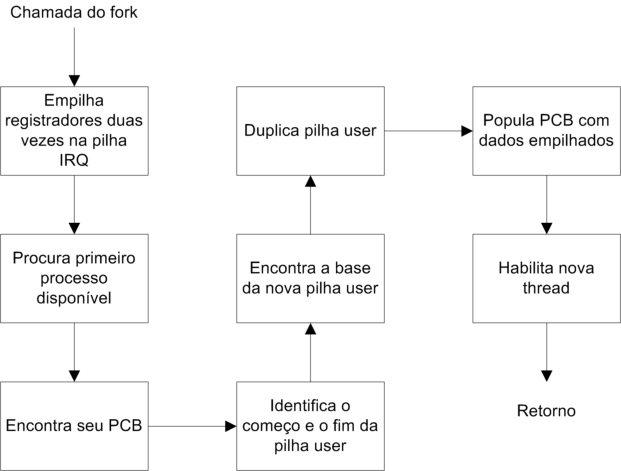
\includegraphics[width=12cm]{figuras/fork.pdf}
\caption{Fluxo de funcionamento do fork. \label{fork}}
\end{figure}

O processo de duplica��o de uma \emph{thread} se inicia com o empilhamento dos registradores de dados (r0 a r12) e do endere�o de retorno (\emph{link register}) por duas vezes, como pode ser visto abaixo. O motivo � que o primeiro empilhamento serve para a restaura��o do estado ao fim do processo de duplica��o e a segunda para a nova c�pia da \emph{thread}, como ser� visto mais � frente. 

\begin{lstlisting}
STMFD 	sp!,{r1-r12,lr}		; Stacks the link register and r1-r12
STMFD 	sp!,{r0-r12}		; Stacks r0-r12
STMFD 	sp!,{lr} 			; Stacks the link register (In a separate instruction
							; to stack it in the top)
\end{lstlisting}

Em segundo lugar, procura-se o primeiro espa�o dispon�vel no vetor de \emph{threads}, o que indica qual dos PCBs est� livre. Na rotina apresentada abaixo, r0 cont�m o id da posi��o sendo procurada e r1 seu endere�o. O loop � feito verificando de posi��o em posi��o, um ponto onde o valor seja 0. Caso se encontre, passa-se ao pr�ximo passo, ao contr�rio, soma-se 1 ao n�mero da \emph{thread} e 4 no endere�o do vetor.

\begin{lstlisting}
	LDR		r1, =thread_array	; r1 = bottom of the thread array address
	MOV		r0,	#1				; r0 = 1
routine_fork_loop
	LDR		r2, [r1]			; r2 = thread array position
	CMP		r2,	#0				; r2 = 0?
	BEQ		pcb_bottom			; If the position is availabe (r2 = 0), go to pcb_bottom
	ADD		r0,	r0,	#1			; r0 = r0 + 1 (next id)
	CMP		r0, #9				; Is this the last thread slot being checked?
	BEQ		fork_fail			; if it is, there is no available slot, go to fork_fail
	ADD		r1,	r1,	#4			; r1 = r1 + 4 (next address)
	B		routine_fork_loop	; Check next slot (go to routine_fork_loop)
\end{lstlisting}

Calcula-se ent�o o endere�o do PCB da \emph{thread} encontrada. A f�rmula, j� vista anteriormente, � $PCB=id \cdot 68$ 

Para se realizar a c�pia da pilha de \emph{user}, h� de se obter tr�s informa��es: a base e o ponteiro da pilha original e a base da nova pilha. O ponteiro � obtido apenas copiando-se o valor do ponteiro de pilha do modo \emph{user}. As bases s�o calculadas a partir da equa��o $0x20000 - (id-1) * 4048$, onde 0x20000 � onde come�a a �rea reservada �s pilhas do modo \emph{user}, id � o n�mero da \emph{thread} cuja base deseja-se obter e 4048 � o tamanho do espa�o reservado para cada pilha.

Com os dados obtidos no passo anterior, pode-se usar a rotina a seguir para se duplicar a pilha:

\begin{lstlisting}
LDR		r6,	[r4]			; r6 = original stack data
STR		r6, [r5]			; Stores data in new stack (stack_top = r6)
CMP		r4,	r3				; Is this the top of the stack? (r4 == r3?)
BEQ		build_new_pcb		; if it is, branch to build_new_pcb 
SUB		r5,	r5,	#4			; if not, go to next space in the new stack (r5 = r5 - 4)
SUB		r4,	r4,	#4			; and next data in the original stack (r4 = r4 - 4)
B		loop_stack_copy		; restart sequence (go to loop_stack_copy)
\end{lstlisting}

O registrador r6 serve como mem�ria intermedi�ria para a c�pia. r4 cont�m o endere�o que est� sendo copiado, e � incrementado de 4 em 4 at� chegar ao seu topo, enquanto r5 guarda o endere�o equivalente da nova pilha, que tamb�m � incrementado de 4 em 4.

Finalmente, se come�a a construir o novo PCB. Na posi��o que guarda o registrador de estado, guarda-se o valor 0x10, que indica que a \emph{thread} deve ser iniciada em modo \emph{user}. O ponteiro de pilha foi obtido no passo anterior, vindo no registrador r5. Tanto o endere�o de retorno do modo \emph{user} quanto o do modo \emph{IRQ} s�o o mesmo, e coloca-se o endere�o inicial da rotina que se quer executar. A c�pia dos valores dos registradores r0 a r12 se d� atrav�s de um loop, como pode-se observar abaixo.

\begin{lstlisting}
; Copy registers
	MOV		r3,	#0		; r3 = 0
	MOV		r4, #12		; r4 = 12
registers_loop
	ADD		r2,	r2,	#4		; r2 = r2 + 4 (Next PCB register space)
	LDMFD	sp!, {r5}		; Restore register from the stack to r5
	STR		r5, [r2]		; Store register in the PCB
	CMP		r3,	r4			; r12 was copied? (r3 == r4?)
	BEQ 	enable_thread	; If yes, go to enable_thread
	ADD		r3,	r3,	#1		; r3 = r3 + 1 (Next register)
	B		registers_loop	; Copy next register
\end{lstlisting}

r2 cont�m o endere�o do PCB onde os dados ser�o colocados, r5 funciona como intermedi�ria entre a pilha e a mem�ria, r4 cont�m o valor final da itera��o e r3 o \emph{id} do registrador sendo copiado.

O �ltimo passo antes de se retornar � execu��o do programa � a habilita��o do programa no vetor de \emph{threads}.


%-------------------------------------------
% System call EXEC
%-------------------------------------------
\subsection{exec}

A chamada de sistema \emph{exec} � respons�vel por substituir a imagem n�cleo de um processo pela imagem do programa passado como argumento \cite{Tanenbaum2000}.

Nos sistemas operacionais tradicionais, como o Linux ou o Minix, o \emph{exec} � utilizado para iniciar um novo programa no mesmo ambiente do programa que executa a chamada de sistema. Normalmente o \emph{exec} � utilizado na cria��o de um novo processo da seguinte maneira: um processo j� existente se duplica atrav�s da chamada de sistema \emph{fork}. O processo filho tem, ent�o, seu c�digo substitu�do pelo c�digo que deve ser executado atrav�s da chamada de sistema \emph{exec}, que permite ao processo filho assumir seu pr�prio conte�do, apagando de si o conte�do do processo pai.

No KinOS, para que um \emph{thread} passe a executar outro programa, � necess�rio reinicializar o seu PCB, isso � feito pela chamada de sistema \emph{exec}.

Existem 4 principais entradas do PCB que necessitam ser reinicializadas: 

\begin{itemize}
\item o \emph{program counter} (PC - R13);
\item o \emph{link register} (LR - R14);
\item o \emph{stack pointer} (SP - R15);
\item e o \emph{saved processor status register} (SPSR).
\end{itemize}

Para reinicializar essas entradas, de forma que a \emph{thread} passe � executar um novo programa, primeiro � necess�rio calcular o in�cio do PCB da \emph{thread} correspondente.

A rotina \emph{exec}, recebe como par�metros o id da \emph{thread} que ser� alterada e o ponteiro para a fun��o/programa que pretende-se executar, como mostrado a seguir:


\begin{lstlisting}
	void exec(int process_id, pt2Task process_addr);
\end{lstlisting}

Assim para calcular o endere�o inicial do PCB, obt�m-se o endere�o inicial da �rea reservada para armazenar todos os PCBs, a \textbf{process\_control\_block}, e adiciona-se � esta o valor de 68 multiplicado por \textbf{process\_id}, visto que cada PCB ocupa um espa�o de 68 endere�os de mem�ria como mencionado na sess�o \ref{sub:PCB}. O c�digo respons�vel por calcular o PCB � apresentado a baixo:

\begin{lstlisting}
  LDR r3, =process_control_block  ; r3 = the start address of the PCB area
  MOV r4,#68         ; r4 = 68 (space for each process in the PCB)
  MUL r5,r1,r4       ; r5 = (task id) * 68
  ADD r3,r3,r5       ; r3 = PCB start address + r5
\end{lstlisting}

Em seguida, calculado o endere�o inicial do PCB, altera-se suas entradas da seguinte maneira:

\begin{itemize}
\item LR (PCB[-4]) e PC (PCB[-64]) recebem o endere�o da primeira instru��o do novo programa (\textbf{process\_addr}).

\begin{lstlisting}
PCB[-4] = process_addr;
PCB[-64] = process_addr;
\end{lstlisting}

\item SP (PCB[-8]) recebe o endere�o de in�cio da pilha da \emph{thread}, fazendo com que esta seja zerada. Para cada pilha de \emph{thread}, 4048 bytes s�o reservados. 

\begin{lstlisting}
PCB[-8] =  in�cio da pilha do modo usu�rio - (4048 * thread id);
\end{lstlisting}

\item SPSR (PCB[-68]) recebe 0x10, pois os programas devem rodar no modo usu�rio.

\begin{lstlisting}
PCB[-68] = 0x10;
\end{lstlisting}

\end{itemize}

Finalmente, ap�s alterar as entradas mostradas a cima, a \emph{thread} come�a a executar o novo programa.



%-------------------------------------------
% System call EXIT
%-------------------------------------------
\subsection{exit}

A chamada de sistema \emph{exit} � respons�vel por finalizar um processo, liberando espa�o de mem�ria para a execu��o de um novo processo \cite{Tanenbaum2000}.

No KinOS isso � realizado apenas colocando como desativado (igual � 0) o byte na lista de processos que  corresponde a \emph{thread} que se deseja finalizar. 

Para isso a rotina \emph{exit} recebe como par�metro o id da \emph{thread} a ser terminada.

\begin{lstlisting}
	void exit(int process_id);
\end{lstlisting}

%-------------------------------------------
% Shell
%-------------------------------------------
\section{Shell}

Com o desenvolvimento do microkernel e de suas system calls, torna-se necess�rio o desenvolvimento de outro ramo do projeto, destinado a permitir a intera��o do usu�rio com o Sistema Operacional. Essa intera��o � feita por um editor de linha de comando, tamb�m conhecido por Shell.

Na inicializa��o do microkernel, o Shell � o primeiro processo criado no sistema. Desse momento em diante, cabe ao usu�rio solicitar a execu��o ou o t�rmino de outras \emph{threads}. Al�m disso, o Shell permite a visualiza��o das diferentes \emph{threads} em execu��o no sistema.

\subsection{Comunica��o via terminal}

O Shell, para fazer a intera��o com o usu�rio, utiliza a porta serial COM0 (de uso geral) conectada a uma segunda porta serial da m�quina host. A porta COM1 (Debug) deve permanecer conectada, pois o Angel mant�m comunica��es atrav�s dela com o AXD (descrito na se��o \ref{axd}) durante a execu��o do KinOS, como ilustrado na figura \ref{e7t_comm}.

\begin{figure}[!ht]
\centering 
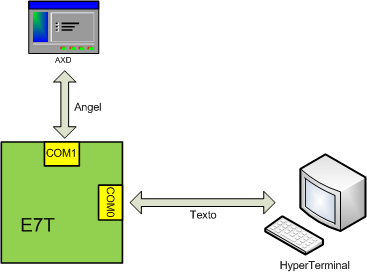
\includegraphics[height=8cm]{figuras/e7t_comm.png}
\caption{Comunica��o da Evaluator-7T em cada porta serial.\label{e7t_comm}}
\end{figure}

% Configuracao e comunicacao da COM0
\subsection{Configura��o e uso da COM0}

Para utilizar a porta COM0 da Evaluator-7T, � preciso configurar um conjunto de registradores mapeados em mem�ria relativos � UART0 do microcontrolador. A tabela \ref{table:regscom0} lista os registradores usados no projeto e suas respectivas fun��es.

\begin{table}[!ht]
\caption{Registradores mapeados em mem�ria da UART0 \cite{uControllerUserManual} }
\centering
\begin{tabular}{| c | c | c | c |}
\hline  \textbf{Registrador} & \textbf{Offset} & \textbf{R/W} & \textbf{Descri��o}  \\ 
\hline  ULCON0 & 0xD000 & R/W & Registrador de controle de linha \\ 
\hline  UCON0 & 0xD004 & R/W & Registrador de controle \\ 
\hline  USTAT0 & 0xD008 & R & Registrador de status \\ 
\hline  UTXBUF0 & 0xD00C & W & Registrador de buffer de transmiss�o \\ 
\hline  URXBUF0 & 0xD010 & R & Registrador de buffer de recep��o \\ 
\hline  UBRDIV0 & 0xD014 & R/W & Registrador de divisor de taxa de transmiss�o \\ 
\hline 
\end{tabular}
\label{table:regscom0}
\end{table}

A coluna \emph{offset} da tabela \ref{table:regscom0} indica o endere�o de mem�ria do registrador a partir do endere�o inicial, que � 0x03FF0000. Esse endere�o � o do registrador SYSCFG, de configura��o de sistema, o qual encabe�a a lista dos registradores mapeados em mem�ria.

Na inicializa��o da COM0, escreve-se nos registradores ULCON0, UCON0 e UBRDIV0. Os valores a serem colocados em cada um seus respectivos significados est�o descritos na tabela \ref{table:regscom0init}.

\begin{table}[!ht]
\caption{Registradores mapeados em mem�ria da UART0 \cite{uControllerUserManual} }
\centering
\begin{tabular}{| c | c | p{7cm} |}
\hline  \textbf{Registrador} & \textbf{Valor} & \textbf{Significado} \\ 
\hline  ULCON0 & 0x03 & 8 bits de dados, 1 bit de parada, sem paridade, fonte de clock interna e modo de opera��o normal. \\ 
\hline  UCON0 & 0x09 & Rx e Tx por requisi��o de interrup��o, sem gera��o de interrup��o por status de recep��o, sem loop-back. \\ 
\hline  UBRDIV0 & 0xA20 & Define a taxa de transmiss�o em 9600 bauds. \\ 
\hline 
\end{tabular}
\label{table:regscom0init}
\end{table}

Inicializada a COM0, a transmiss�o de um caractere por ela � feita da seguinte maneira: observa-se o conte�do do bit 6 de USTAT0. Quando este � igual a 1, significa que UTXBUF0 n�o cont�m dados v�lidos e, portanto, pode-se escrever nele o caractere que pretende-se enviar. Em seguida, coloca-se o caractere desejado em UTXBUF0. A l�gica do controlador UART do microcontrolador se encarrega de enviar o dado para o terminal.

A recep��o de caracteres � feita de forma similar: dessa vez, a verifica��o � feita no bit 5 de USTAT0, o qual � igual a 1 quando cont�m dados v�lidos recebidos pela porta serial. Quando isso acontece, copia-se o conte�do de URXBUF0 para uma vari�vel no programa do tipo \emph{char}.

\subsection{Funcionalidades do Shell}

O editor de linha de comando do KinOS possui tr�s funcionalidades b�sicas: listar \emph{threads} ativas (\emph{ps}), inicializar novas \emph{threads} (\emph{start}) e encerrar \emph{threads} ativas (\emph{end}). As sintaxes de cada comando s�o, respectivamente:

\begin{lstlisting}
ps

start <nome da thread>

end <nome da thread>
\end{lstlisting}

O comando \emph{ps} utiliza o vetor de threads do sistema operacional para saber quais \emph{threads} est�o ativas. A partir da�, buscam-se as informa��es sobre cada \emph{thread} ativa em seu respectivo PCB. Essas informa��es s�o, ent�o, listadas ao usu�rio.

O comando \emph{start} utiliza as system calls \emph{fork} e \emph{exec} para iniciar novas \emph{threads} no sistema. O usu�rio deve fornecer o nome da \emph{thread} como par�metro do comando. Cada \emph{thread} que pode ser disparada dentro do KinOS j� est� definida dentro do c�digo-fonte, e cada um de seus nomes tamb�m j� est� definido.

O comando \emph{end} � similar ao \emph{start}. Dessa vez, o comando recebe o nome de uma \emph{thread} ativa no sistema e utiliza a system call \emph{exit} para encerr�-la.

\section{\emph{Mutex}}

O \emph{mutex} ou exclus�o m�tua, � uma t�cnica usada para evitar que dois processos tenham acesso a um mesmo espa�o de mem�ria. Seu funcionamento � baseado em uma vari�vel que pode ter apenas dois valores, 0 ou 1. Caso ela seja 0, ela indica que a �rea cr�tica pode ser acessada e 1 caso contr�rio. No caso de um processo n�o obter acesso, ele fica em espera ativa, at� que o processo que o bloqueou o desfa�a.

No exemplo que � dado no KinOS, tem-se duas fun��es que realizam o travamento e o destravamento do \emph{mutex} e a vari�vel semaphore, que guarda o valor do \emph{mutex}. A primeira fun��o se chama \verb|mutex_gatelock|, que pode ser observada abaixo.

\begin{lstlisting}
void mutex_gatelock (void) {
	__asm {
		spin:
		mov		r1, &semaphore
		mov		r2, #1
		swp		r3,r2,[r1]
		cmp		r3,#1
		beq		spin
	}
}
\end{lstlisting}

r1 recebe o endere�o da vari�vel semaphore, e r2 recebe 1. A fun��o at�mica swp � que permite o correto funcionamento do \emph{mutex}: em uma instru��o indivis�vel, o conte�do de semaphore � colocado em r3, e 1 � colocado em semaphore. Com isso, � imposs�vel que haja uma interrup��o entre estas duas a��es, o que poderia arruinar uma rotina de \emph{mutex}. Finalmente, caso semaphore j� estivesse ativo quando chamado, a rotina seria executada novamente.

\begin{lstlisting}
void mutex_gateunlock (void)  {
	__asm  {
		mov		r1, &semaphore
		mov		r2, #0
		swp		r0,r2,[r1]
	}
}
\end{lstlisting}

O destravamento � feito de modo similar, com a mesma instru��o. S� que neste caso, o valor 0 � colocado em semaphore.

Por�m, as rotinas apresentadas n�o s�o chamadas diretamente. Usa-se as chamadas abaixo.

\begin{lstlisting}
#define WAIT 		while (semaphore==1) {} mutex_gatelock(); 
#define SIGNAL 		mutex_gateunlock(); 	
\end{lstlisting}

O motivo � que ao se usar o \verb|WAIT| quando o \emph{mutex} est� ativo, faz com que o programa entre em uma espera ativa.

\section{Processos} \label{cap:processos}

O kernel pode lidar com no m�ximo nove processos, nomeados de task1 a task9 no arquivo tasks.c. Como eles n�o t�m �rea de dados pr�pria, n�o pode-se cham�-los de processos. A implica��o de se ter uma �rea de dados em comum � que todos os processos que rodam um mesmo programa compartilham os valores das vari�veis. O mais correto, portanto, seria o cham�-os de threads.

Criamos algums programas exemplo que se utilizam dos perif�ricos da placa. 

TODO\ldots (Fazer c�digo antes)

\section{Inspira��o}

Grande parte do c�digo foi baseada do c�digo presente nos exemplos inclu�dos no CD de demonstra��o da placa, desenvolvido por Andrew N. Sloss. O principal deles, � o c�digo \emph{mutex}, de onde foi baseado o chaveamento de processos, a fun��o de mutex e as rotinas de manipula��o de hardware. Eis a inspira��o de cada uma das partes do projeto:

\paragraph{Chaveamento de processos} O chaveamento de processos original, contido no projeto mutex era de apenas duas threads. Modifica��es foram realizadas para fazer com que o n�mero de processos passasse de duas para nove.

\paragraph{Inicializa��o} A inicializa��o foi baseada no c�digo do mutex, mas grandes altera��es foram feitas e pouqu�ssimas coisas ainda restam do c�digo original

\paragraph{Shell} O c�digo foi baseado no exemplo da porta serial e tamb�m no Sistema Operacional ISOS \cite{ISOSPage}.

\paragraph{Interrup��o de hardware} O c�digo foi baseado no exemplo do mutex, mas grandes altera��es foram realizadas

\paragraph{Interrup��o de software} Foi baseado no exemplo SWI, tamb�m contido no CD da placa

\paragraph{Rotinas de manipula��o de perif�ricos} As rotinas foram praticamente copiadas do c�digo do mutex, que utiliza todas elas

\paragraph{Chamadas de sistema} Todas as chamadas de sistema foram inteiramente desenvolvidas durante o projeto

\paragraph{Mutex} O c�digo do mutex foi inteiramente copiado do exemplo com o mesmo nome
